\subsection{Gestion des utilisateurs}
\subsubsection{Les différents types d'utilisateurs}
L'application est structurée autours de trois niveaux hiérarchiques pour les utilisateurs :
\begin{itemize}
  \itemperso{Visiteur}Il s'agit du niveau avec le moins d'accréditations possibles. Cet utilisateur correspond à une personne lambda naviguant sur le site, sans être client de Centrale-Télécom.
  \itemperso{Client}Ce niveau permet de représenter les clients qui viennent consulter leurs factures, leurs abonnements ou encore les nouvelles offres disponibles.
  \itemperso{Administrateur}Ce grade est celui avec le plus de droit. Il représente les employés de Centrale-Télécom qui ont donc le droit d'éditer les profils, créer des abonnements, des téléphones,...
\end{itemize}
Les clients et les administrateurs sont des profils qui sont détectés après une connexion à la plateforme. Ils sont différenciés au niveau de la base de données via la colonne \texttt{admin} de la table \texttt{utilisateur}, qui est mise à \texttt{TRUE} si l'utilisateur est un administrateur. Une fois la connexion effectuée, on stocke les informations dans la variable globale \texttt{\$\_SESSION}. Le cas des visiteurs correspond alors aux valeurs par défaut pour \texttt{\$\_SESSION}. On retrouve alors les caractéristiques de la Table~\ref{tab:utilisation_session}.

\begin{table}[ht]
  \centering
  \begin{tabular}{ccc}
    \toprule
    \textbf{Type d'utilisateur} & \textbf{Champ \texttt{log\_in}} & \textbf{Champ \texttt{login\_level}} \\
    \midrule
    Visiteur & \texttt{False} & Sans importance (\texttt{False}) \\
    Client   & \texttt{True} & \texttt{False} \\
    Administrateur & \texttt{True} & \texttt{True} \\
    \bottomrule
  \end{tabular}
  \caption{Valeurs stockées dans \texttt{\$\_SESSION} pour les différents profils d'utilisateurs}
  \label{tab:utilisation_session}
\end{table}

Ces grandeurs nous permettent d'adapter les affichages en fonction du type d'utilisateur.

\subsubsection{Connexion et déconnexion}
\subParagraphe{Réalisation des actions}Ces deux actions sont réalisées à partir d'un vue accesible en cliquant sur l'icône \thColor{\faUser}.

\begin{figure}[ht]
  \centering
  \begin{subfigure}{.45\textwidth}
    \centering
    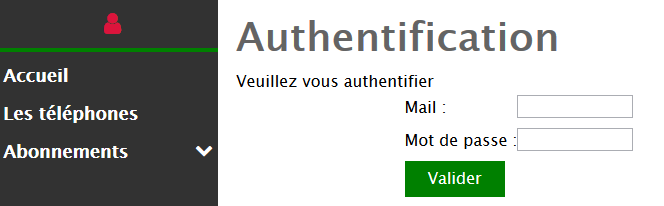
\includegraphics[width=.95\textwidth]{images/Plateforme/connexion}
    \caption{Connexion d'un utilisateur}
    \label{fig:connexion}
  \end{subfigure}\hfill%
  \begin{subfigure}{.45\textwidth}
    \centering
    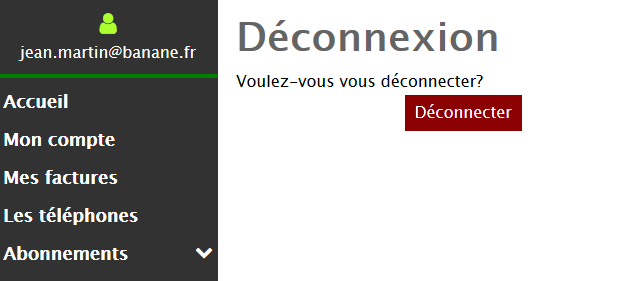
\includegraphics[width=.95\textwidth]{images/Plateforme/deconnexion}
    \caption{Déconnexion d'un utilisateur}
    \label{fig:deconnexion}
  \end{subfigure}
  \caption{Les fenêtres de connexion et déconnexion des utilisateurs}
\end{figure}

Une première vue (Figure~\ref{fig:connexion}) permet aux utilisateurs de se déconnecter. Le principe est usuel, où l'utilisateur va fournir son adresse mail (qui fait office d'identifiant ici) ainsi que son mot de passe. Si les deux concordent, l'utilisateur est connecté, sinon il devra ré-essayer.

Pour la déconnexion, il suffit de se rendre aussi sur cette page (Figure~\ref{fig:deconnexion}), qui propose alors un bouton pour se déconnecter.

\subParagraphe{Différences visuelles}On remarquera également une différence sur la partie haute de la barre de navigation, où l'avatar \faUser{} est en rouge (\thColor{\faUser}) si l'utilisateur n'est pas enregistré et en vert (\textcolor{vertforet}{\faUser}) si l'utilisateur est connecté. De même, quand l'utilisateur est connecté, son adresse mail apparaît sous cette icône.

\subParagraphe{Pour les visiteurs}Un visiteur ne disposant pas de compte, il ne peut se connecter, et n'aura donc accès à aucune vue de celles précisées dans la suite de cette section.

\subsubsection{\'Edition du profil en tant que client}
Un client dispose de la possibilité de voir et éditer les informations de son profil (sauf son statut!) directement par la vue intitulée \og Mon compte\fg. La vue de consultation du profil vous est proposée à la Figure~\ref{fig:vueprofilclient} présente les différentes informations au client, ainsi qu'un bouton d'édition. La vue d'édition associée est présentée à la Figure~\ref{fig:vueeditionclient}.

\begin{figure}[ht]
  \centering
  \begin{subfigure}{.45\textwidth}
    \centering
    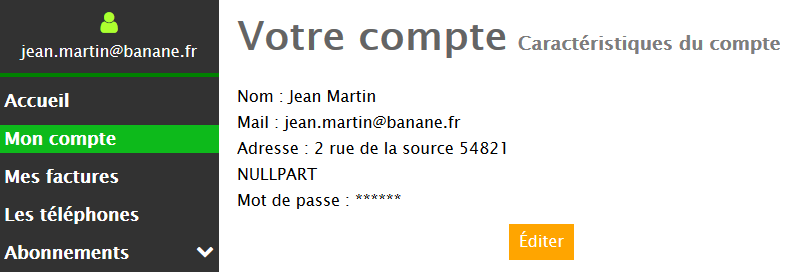
\includegraphics[width=.95\textwidth]{images/Plateforme/vue_profil_client}
    \caption{Vue du profil}
    \label{fig:vueprofilclient}
  \end{subfigure}\hfill%
  \begin{subfigure}{.45\textwidth}
    \centering
    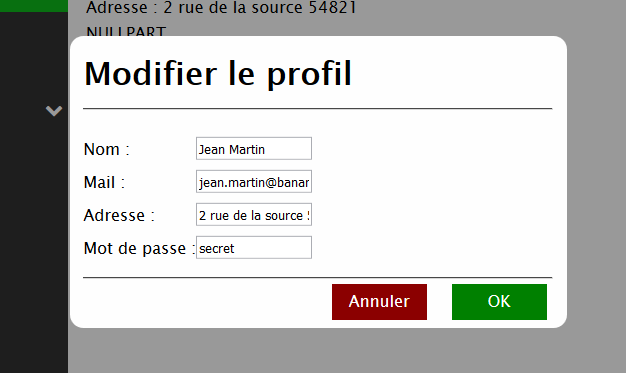
\includegraphics[width=.95\textwidth]{images/Plateforme/vue_edition_profil}
    \caption{\'Edition de son profil}
    \label{fig:vueeditionclient}
  \end{subfigure}
  \caption{Gestion du compte par un client}
\end{figure}

\subsubsection{\'Edition des profils en tant qu'administrateur}
Un administrateur dispose lui de plus de droit. Il peut ainsi voir la liste de tous les utilisateurs inscrits à la plateforme, qu'ils soient administrateurs ou simples clients. On remarquera cependant qu'un administrateur qui consulte cette liste ne peut se voir lui-même, pour éviter une modification involontaire de son profil. Cette vue vous est proposée à la Figure~\ref{fig:listeusers}

\begin{figure}[ht]
  \centering
  \begin{subfigure}{.6\textwidth}
    \centering
    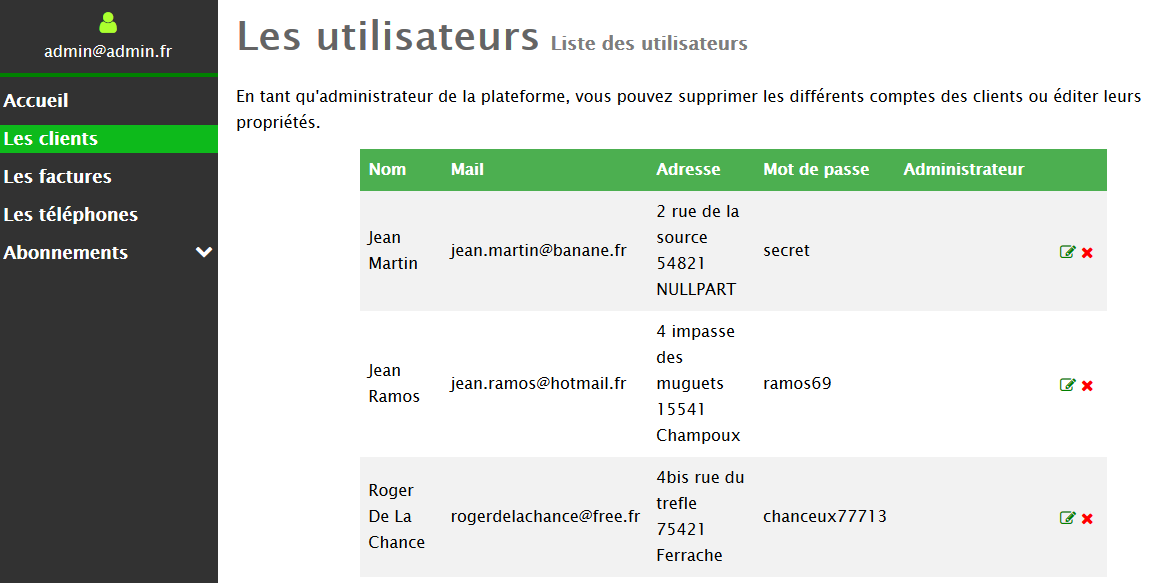
\includegraphics[width=.95\textwidth]{images/Plateforme/liste_utilisateurs}
    \caption{Liste des clients}
    \label{fig:listeusers}
  \end{subfigure}\hfill%
  \begin{subfigure}{.39\textwidth}
    \centering
    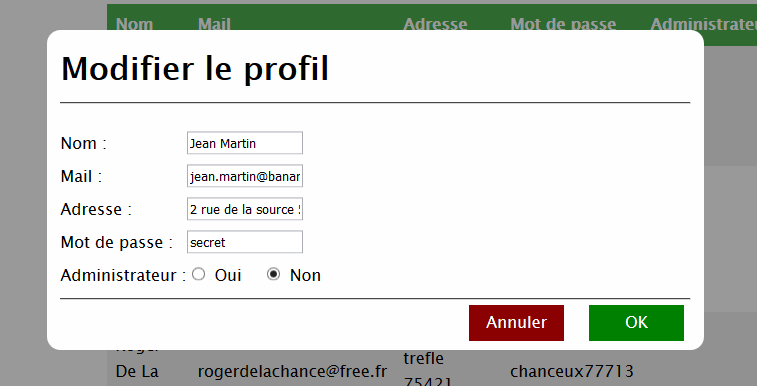
\includegraphics[width=.95\textwidth]{images/Plateforme/vue_edition_clients}
    \caption{\'Edition d'un utilisateur}
    \label{fig:editionuser}
  \end{subfigure}
  \caption{Gestion des comptes clients par un administrateur}
\end{figure}

En effet, outre la liste des utilisateurs, l'administrateur dispose du droit de modifier tous les comptes, que ce soit pour les adresses mails, les noms, les mots de passe ou encore les droits d'accès à la plateforme (administrateur ou non). La fenêtre d'édition est précisée à la Figure~\ref{fig:editionuser} et s'ouvre en cliquant sur une icône \vColor{\faEdit}.

Enfin, l'administrateur peut également supprimer des comptes clients en cliquant sur l'icône \thColor{\faRemove}. On remarquera que dans cette vue, des informations sont apportées à l'administrateur en cas d'échec ou de réussite de sa manipulation.

%%% Local Variables:
%%% mode: latex
%%% TeX-master: "../../Rapport_BDD"
%%% End:
